\section{OUU Tutorial}
\label{sec:ouu_tutorial}

This section walks through a few examples of running OUU. 

\subsection{Example 1: OUU with Discrete Uncertain Parameters Only}

This example has only discrete uncertain parameters and the objective
function is computed from the mean estimation with the scenarios
from a sample file. 
\begin{figure}[H]
\centering 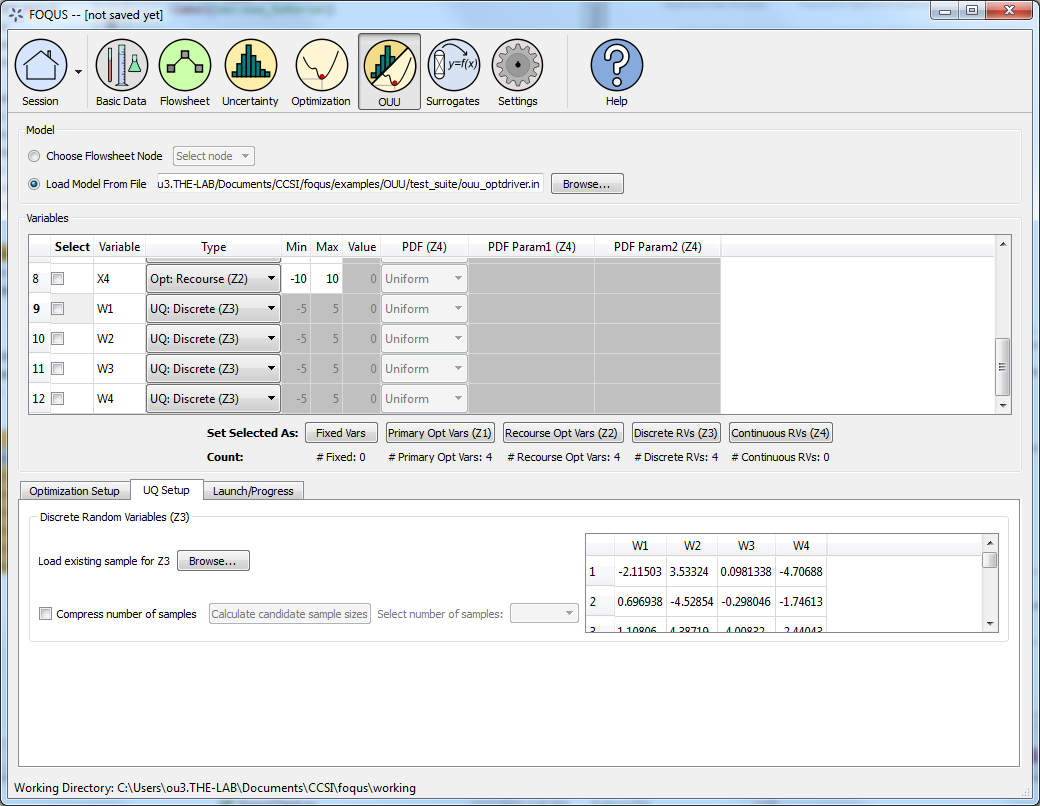
\includegraphics[width=6.0in,height=4.0in,keepaspectratio]{Chapt_ouu/figs/2_OUUExample1}
\caption{OUU Example with Discrete Uncertain Parameters}
\label{fig:ouu_ex1}
\end{figure}

\begin{enumerate}
\item Start FOQUS and click the `OUU' icon.
\item Under `Model', browse and load {\sf examples/OUU/test\_suite/ouu\_optdriver.in}.
\item Under `Variables', set variable $1-4$ as $Z_1$, variable $5-8$ as $Z_2$, and
      variable $9-12$ as $Z_3$.
\item Under `Optimization Setup', select the first objection function (default)
      and select `use model as optimizer' as the `Inner Solver'.
\item Under `UQ Setup' and `Discrete Random Variables', browse the  
      {\sf examples/OUU/test\_suite} directory and load the
      {\sf x3sample.smp} sample file (see Figure \ref{fig:ouu_ex1}).
\item Go to `Launch/Progress' page, click `Run OUU' and see OUU in action.
\end{enumerate}

\subsection{Example 2: OUU with Continuous Uncertain Parameters Only}

This example has only continuous uncertain parameters and the objective
function is computed from the mean estimation with a Latin hypercube
sample of size $200$ for $Z_4$.
\begin{figure}[H]
\centering 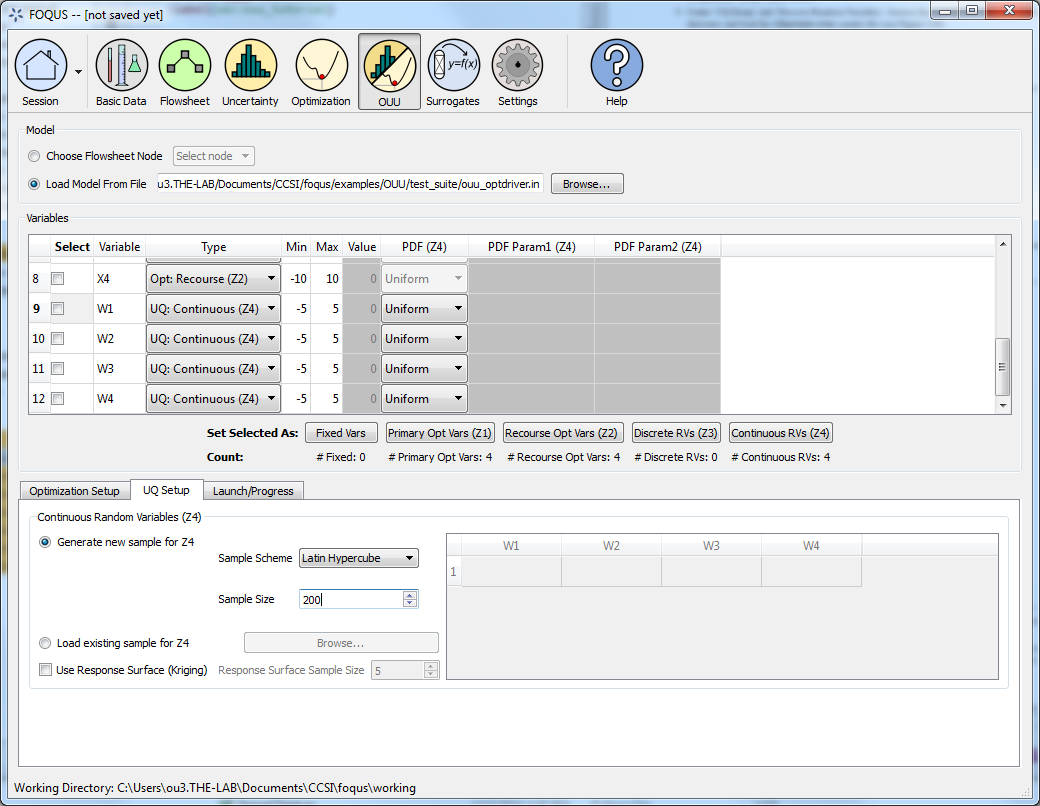
\includegraphics[width=6.0in,height=4.0in,keepaspectratio]{Chapt_ouu/figs/3_OUUExample2}
\caption{OUU Example with Continuous Uncertain Parameters}
\label{fig:ouu_ex2}
\end{figure}

\begin{enumerate}
\item Start FOQUS and click the `OUU' icon.
\item Under `Model', browse and load {\sf examples/OUU/test\_suite/ouu\_optdriver.in}.
\item Under `Variables', set variable $1-4$ as $Z_1$, variable $5-8$ as $Z_2$, and
      variable $9-12$ as $Z_4$.
\item Under `Optimization Setup', select the first objection function (default)
      and select `use model as optimizer' as the `Inner Solver'.
\item Under `UQ Setup' and `Continuous Random Variables', select 
      `Generate new sample for $Z_4$', set `Sample Scheme'
      to `Latin Hypercube' and set sample size to $200$ (see Figure \ref{fig:ouu_ex2}).
\item Go to `Launch/Progress' page, click `Run OUU' and see OUU in action.
\end{enumerate}

\subsection{Example 3: OUU with Continuous Uncertain Parameters and Response Surface}

This example is similar to Example 2 except that response surfaces will be used
on the $Z_4$ sample (that is, the $Z_4$ sample will be used to construct response
surfaces and the means will be estimated from a large sample evaluated on the
response surfaces).

\begin{enumerate}
\item Start FOQUS and click the `OUU' icon.
\item Under `Model', browse and load {\sf examples/OUU/test\_suite/ouu\_optdriver.in}.
\item Under `Variables', set variable $1-4$ as $Z_1$, variable $5-8$ as $Z_2$, and
      variable $9-12$ as $Z_4$.
\item Under `Optimization Setup', select the first objection function (default)
      and select `use model as optimizer' as the `Inner Solver'.
\item Under `UQ Setup' and `Continuous Random Variables', select 
      `Generate new sample for $Z_4$', set `Sample Scheme'
      to `Latin Hypercube' and set sample size to $200$.
\item Under `UQ Setup' and `Continuous Random Variables', check the 
      `Use Response Surface' box (see Figure \ref{fig:ouu_ex2}).
\item Go to `Launch/Progress' page, click `Run OUU' and see OUU in action.
\end{enumerate}

\subsection{Example 4: OUU with Discrete and Continuous Uncertain Parameters}

This example has both discrete and continuous parameters. The discrete scenarios
will be loaded from a sample file. A Latin hypercube sample will be generated for
the continuous variables.
 
\begin{enumerate}
\item Start FOQUS and click the `OUU' icon.
\item Under `Model', browse and load {\sf examples/OUU/test\_suite/ouu\_optdriver.in}.
\item Under `Variables', set variable $1-4$ as $Z_1$, variable $5-8$ as $Z_2$, 
      variable $9$ as $Z_3$, and variable $10-12$ as $Z_4$.
\item Under `Optimization Setup', select the first objection function (default)
      and select `use model as optimizer' as the `Inner Solver'.
\item Under `UQ Setup' and `Discrete Random Variables', browse the
      {\sf examples/OUU/test\_suite} directory and load the
      {\sf x3sample4.smp} sample file.
\item Under `UQ Setup' and `Continuous Random Variables', select
      `Generate new sample for $Z_4$', set `Sample Scheme' to Latin hypercube
      and set `Sample Size' to $100$.
\item Go to `Launch/Progress' page, click `Run OUU' and see OUU in action.
\end{enumerate}

\subsection{Example 5: OUU with Mixed Uncertain Parameters and Response Surface}

This example is similar to Example 4 except that response surfaces will be used
to estimate the means for the continuous uncertain variables.

\begin{enumerate}
\item Start FOQUS and click the `OUU' icon.
\item Under `Model', browse and load {\sf examples/OUU/test\_suite/ouu\_optdriver.in}.
\item Under `Variables', set variable $1-4$ as $Z_1$, variable $5-8$ as $Z_2$, 
      variable $9$ as $Z_3$, and variable $10-12$ as $Z_4$.
\item Under `Optimization Setup', select the first objection function (default)
      and select `use model as optimizer' as the `Inner Solver'.
\item Under `UQ Setup' and `Discrete Random Variables', browse the
      {\sf examples/OUU/test\_suite} directory and load the
      {\sf x3sample4.smp} sample file.
\item Under `UQ Setup' and `Continuous Random Variables', select
      `Generate new sample for $Z_4$', set `Sample Scheme' to Latin hypercube
      and set `Sample Size' to $100$.
\item Under `UQ Setup' and `Continuous Random Variables', check the
      `Use Response Surface' box.
\item Go to `Launch/Progress' page, click `Run OUU' and see OUU in action.
\end{enumerate}

\subsection{Example 6: OUU with User-provided Samples and Response Surface}

This example is similar to Example 4 except that a sample for $Z_4$ will be
used (instead of the Latin hypercube sample generated internally).

\begin{enumerate}
\item Start FOQUS and click the `OUU' icon.
\item Under `Model', browse and load {\sf examples/OUU/test\_suite/ouu\_optdriver.in}.
\item Under `Variables', set variable $1-4$ as $Z_1$, variable $5-8$ as $Z_2$, 
      variable $9$ as $Z_3$, and variable $10-12$ as $Z_4$.
\item Under `Optimization Setup', select the first objection function (default)
      and select `use model as optimizer' as the `Inner Solver'.
\item Under `UQ Setup' and `Discrete Random Variables', browse the
      {\sf examples/OUU/test\_suite} directory and load the
      {\sf x3sample4.smp} sample file.
\item Under `UQ Setup' and `Continuous Random Variables', check `Load existing
      sample for $Z_4$' and load the $Z_4$ sample 
      {\sf examples/OUU/test\_suite/x4sample4.smp}.
\item Go to `Launch/Progress' page, click `Run OUU' and see OUU in action.
\end{enumerate}

\subsection{Example 7: OUU with Large User-provided Samples and Response Surface}

This example is similar to Example 5 except that a sample for $Z_4$ is provided
(instead of generated internally).

\begin{enumerate}
\item Start FOQUS and click the `OUU' icon.
\item Under `Model', browse and load {\sf examples/OUU/test\_suite/ouu\_optdriver.in}.
\item Under `Variables', set variable $1-4$ as $Z_1$, variable $5-8$ as $Z_2$, 
      and variable $9-12$ as $Z_4$.
\item Under `Optimization Setup', select the first objection function (default)
      and select `use model as optimizer' as the `Inner Solver'.
\item Under `UQ Setup' and `Continuous Random Variables', check `Load existing
      sample for $Z_4$' and load the $Z_4$ sample 
      {\sf examples/OUU/test\_suite/x4sampleLarge.smp} ($10000$ sample points).
\item Under `UQ Setup' and `Continuous Random Variables', check
      `Use Response Surface' and set `Sample Size' to $100$.
\item Go to `Launch/Progress' page, click `Run OUU' and see OUU in action.
\end{enumerate}
